\chapter{Conceitos Básicos}
\label{chap:conceitosbasicos}

Aprendizado de máquina é um dos campos de pesquisa da inteligência artificial e por sua vez da ciência da computação.
Esta área de estudos se concentra na pesquisa e desenvolvimento de algoritmos que possam aprender tarefas automaticamente.
Tipicamente estes algoritmos geram um \textit{modelo matemático} a partir de um ou mais conjuntos de dados.
O modelo é então responsável por desempenhar a tarefa, ou seja, não é necessário escrever um programa para tanto.
Aprendizado de máquina tem inúmeras aplicações, entre elas podemos citar filtros de spam, reconhecimento ótico de caracteres, motores de busca, visão computacional, entre outras.

\section{Aprendizado Supervisionado}

Aprendizado supervisionado é inspirado na ideia de aprendizado por exemplos.
Isto é, uma grande quantidade de exemplos é fornecida para o algoritmo no intuito de fazê-lo aprender.
Todos os exemplos devem ter o mesmo formato.
Cada um deles é composto por dois ou mais atributos, sendo que um dos atributos deve ser o alvo da tarefa de aprendizado.
Os demais atributos devem constituir informações relevantes que permitam ao algoritmo aprender a tarefa.
De forma geral temos que um conjunto com \textit{N} exemplos é da forma $ \{(x_1, y_1), ..., (x_N,\; y_N)\} $ tal que $x_i$ representa o conjunto de atributos informativos do exemplo e $y_i$ é seu atributo alvo.

\begin{figure}[h!]
  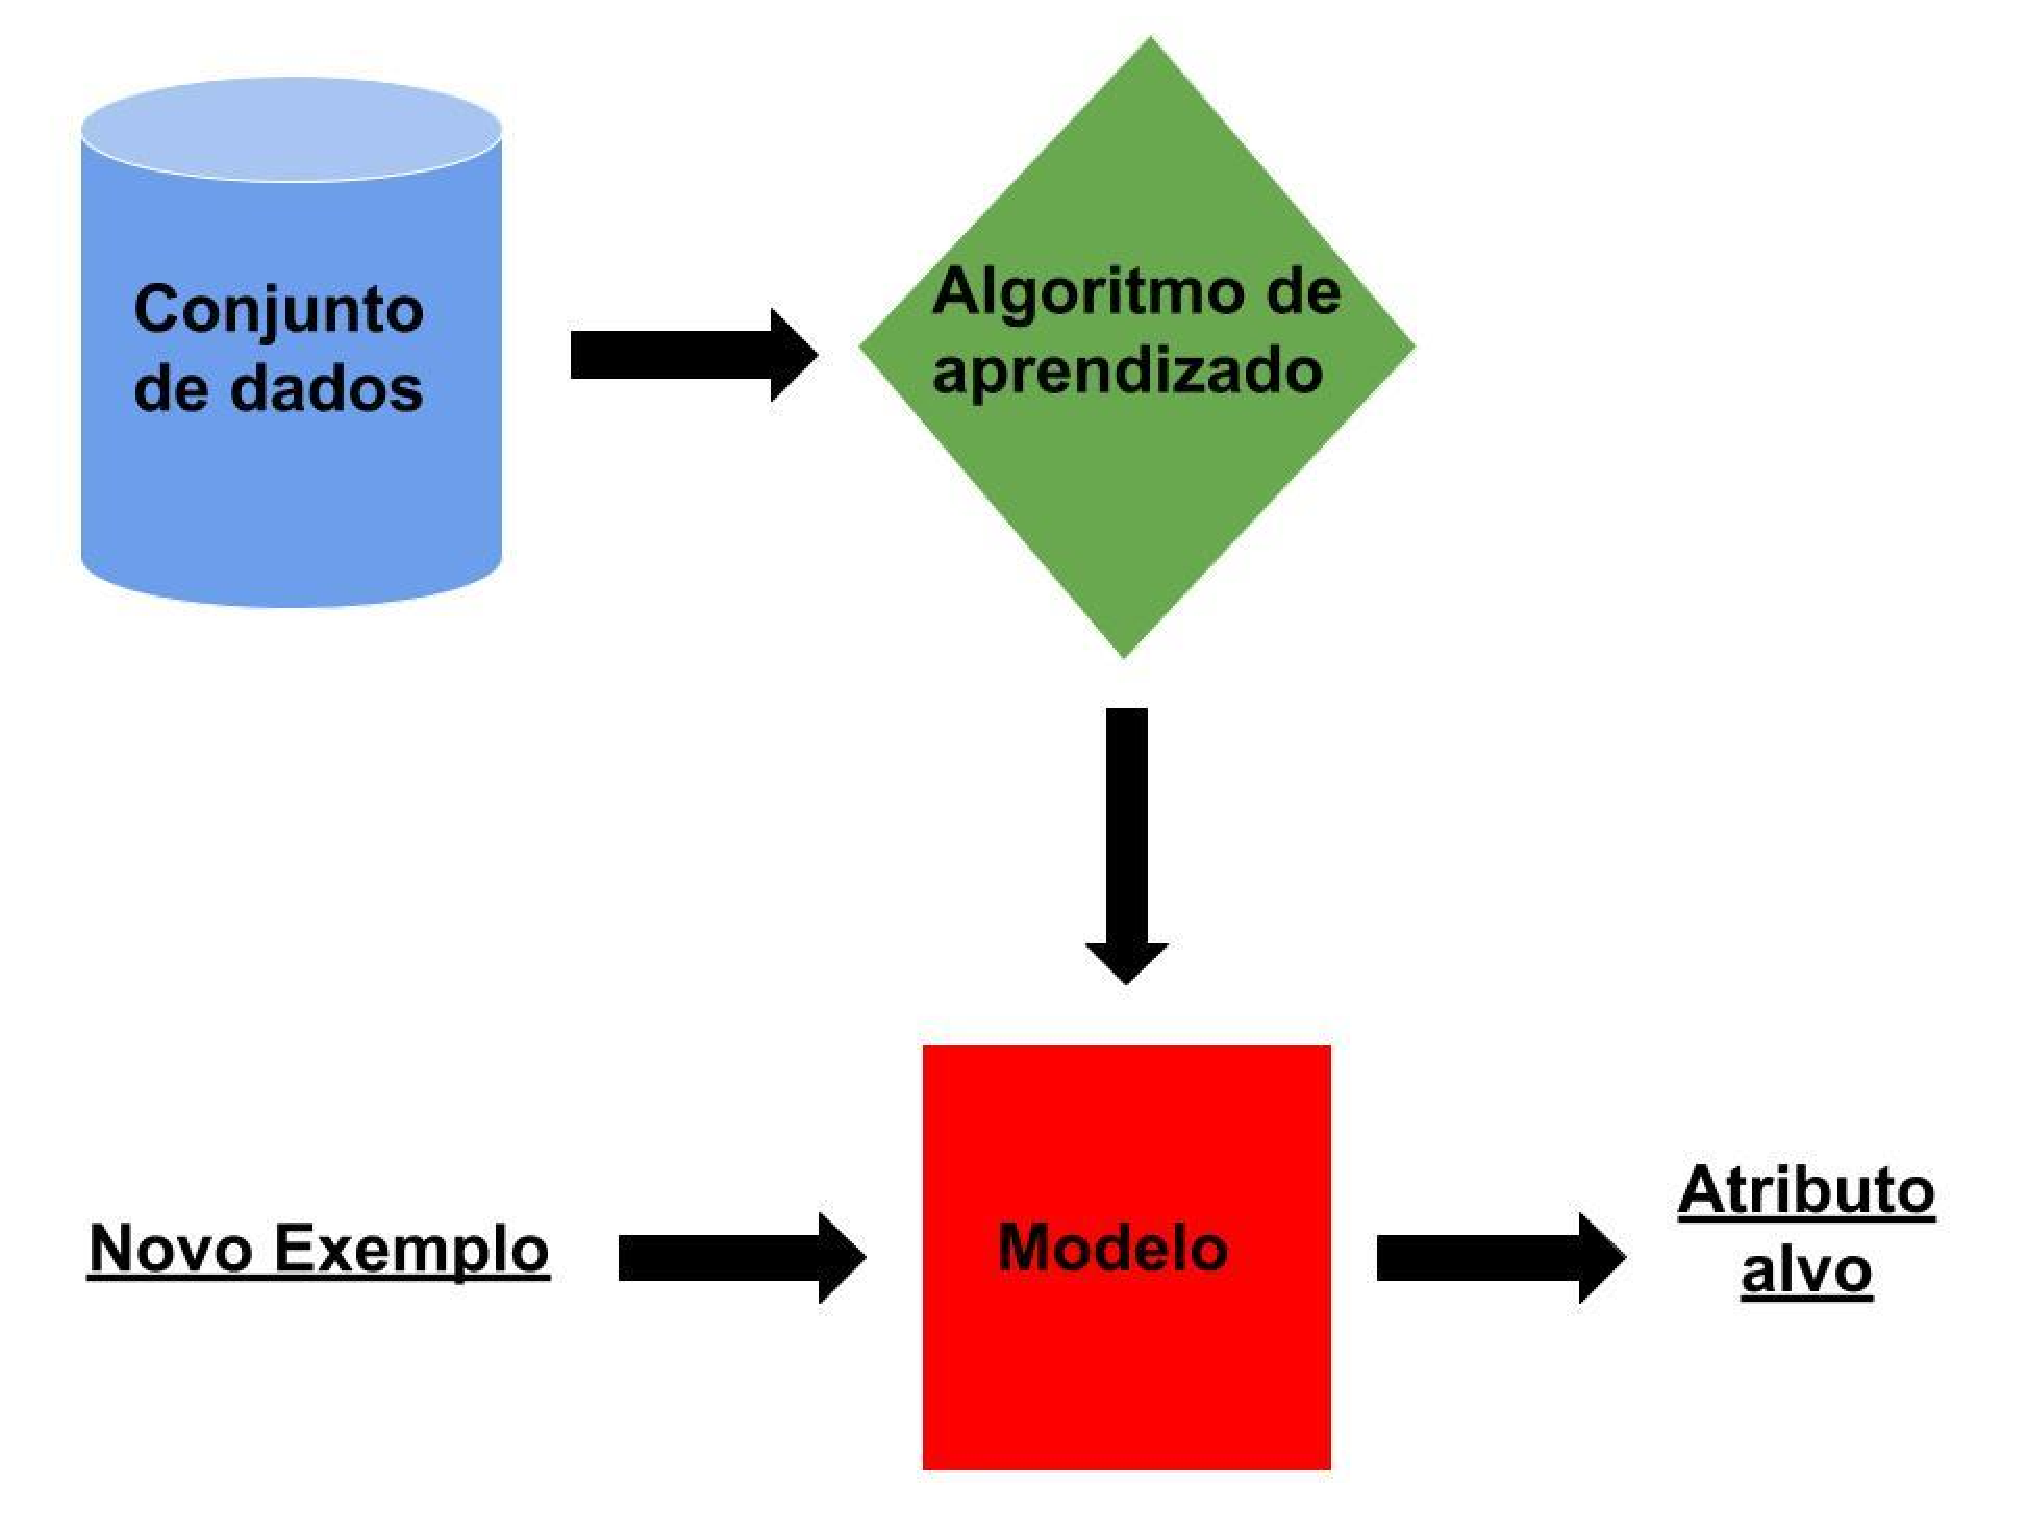
\includegraphics[width=\linewidth]{images/conceitosbasicos01.eps}
  \caption{Fluxo do aprendizado supervisionado para classificação}
  \label{fig:conceitosbasicos01}
\end{figure}

O algoritmo de aprendizado deve gerar uma função $g: X \to Y$, onde \textit{X} é o conjunto de entrada e \textit{Y} o conjunto de saída.
Uma vez que processou os exemplos, o algoritmo gera um modelo que representa a função \textit{g}.
Por fim, dados que ainda não foram vistos, desprovidos do atributo alvo, podem ser submetidos ao modelo.
Com isso, ele pode executar automaticamente a tarefa para a qual foi treinado, e.g. determinar a qual classe o dado inédito pertence.
Veja na Figura \ref{fig:conceitosbasicos01} um diagrama que ilustra o processo de aprendizado supervisionado.

Para exemplificar como funciona o aprendizado supervisionado, consideremos o problema da Figura \ref{fig:conceitosbasicos02}.
Neste queremos um modelo capaz de diferenciar entre círculos e triângulos.
Ou seja, temos um problema de classificação binária.
Para resolvê-lo precisamos de um modelo que funcione como um separador linear.
O algoritmo utilizado para gerar o modelo deve então aprender uma função \textit{f(x)} que mapeia o vetor de entrada \textit{x} em um único valor de saída. Esta função pode ser definida como:

\begin{equation*}

\centering

f(x) =
        \begin{cases}

        1 & \text{se }w \cdot x + b > 0\\
        0 & \text{caso contrário}

        \end{cases}

\end{equation*}

onde,
\begin{itemize}
\item Os valores de saída de \textit{f(x)} representam a resposta do classificador, por exemplo o valor 0 pode indicar um círculo e o valor 1 um triângulo
\item \textit{x} é um vetor de números reais que representam os valores de atributos de entrada, no exemplo podem ser as coordenadas dos centros de cada círculo e triângulo
\item \textit{w} é um vetor de números reais que representam os pesos conferidos aos atributos pelo algoritmo de aprendizado
\item \textit{b} é uma constante de bias
\end{itemize}

\begin{figure}[h!]
  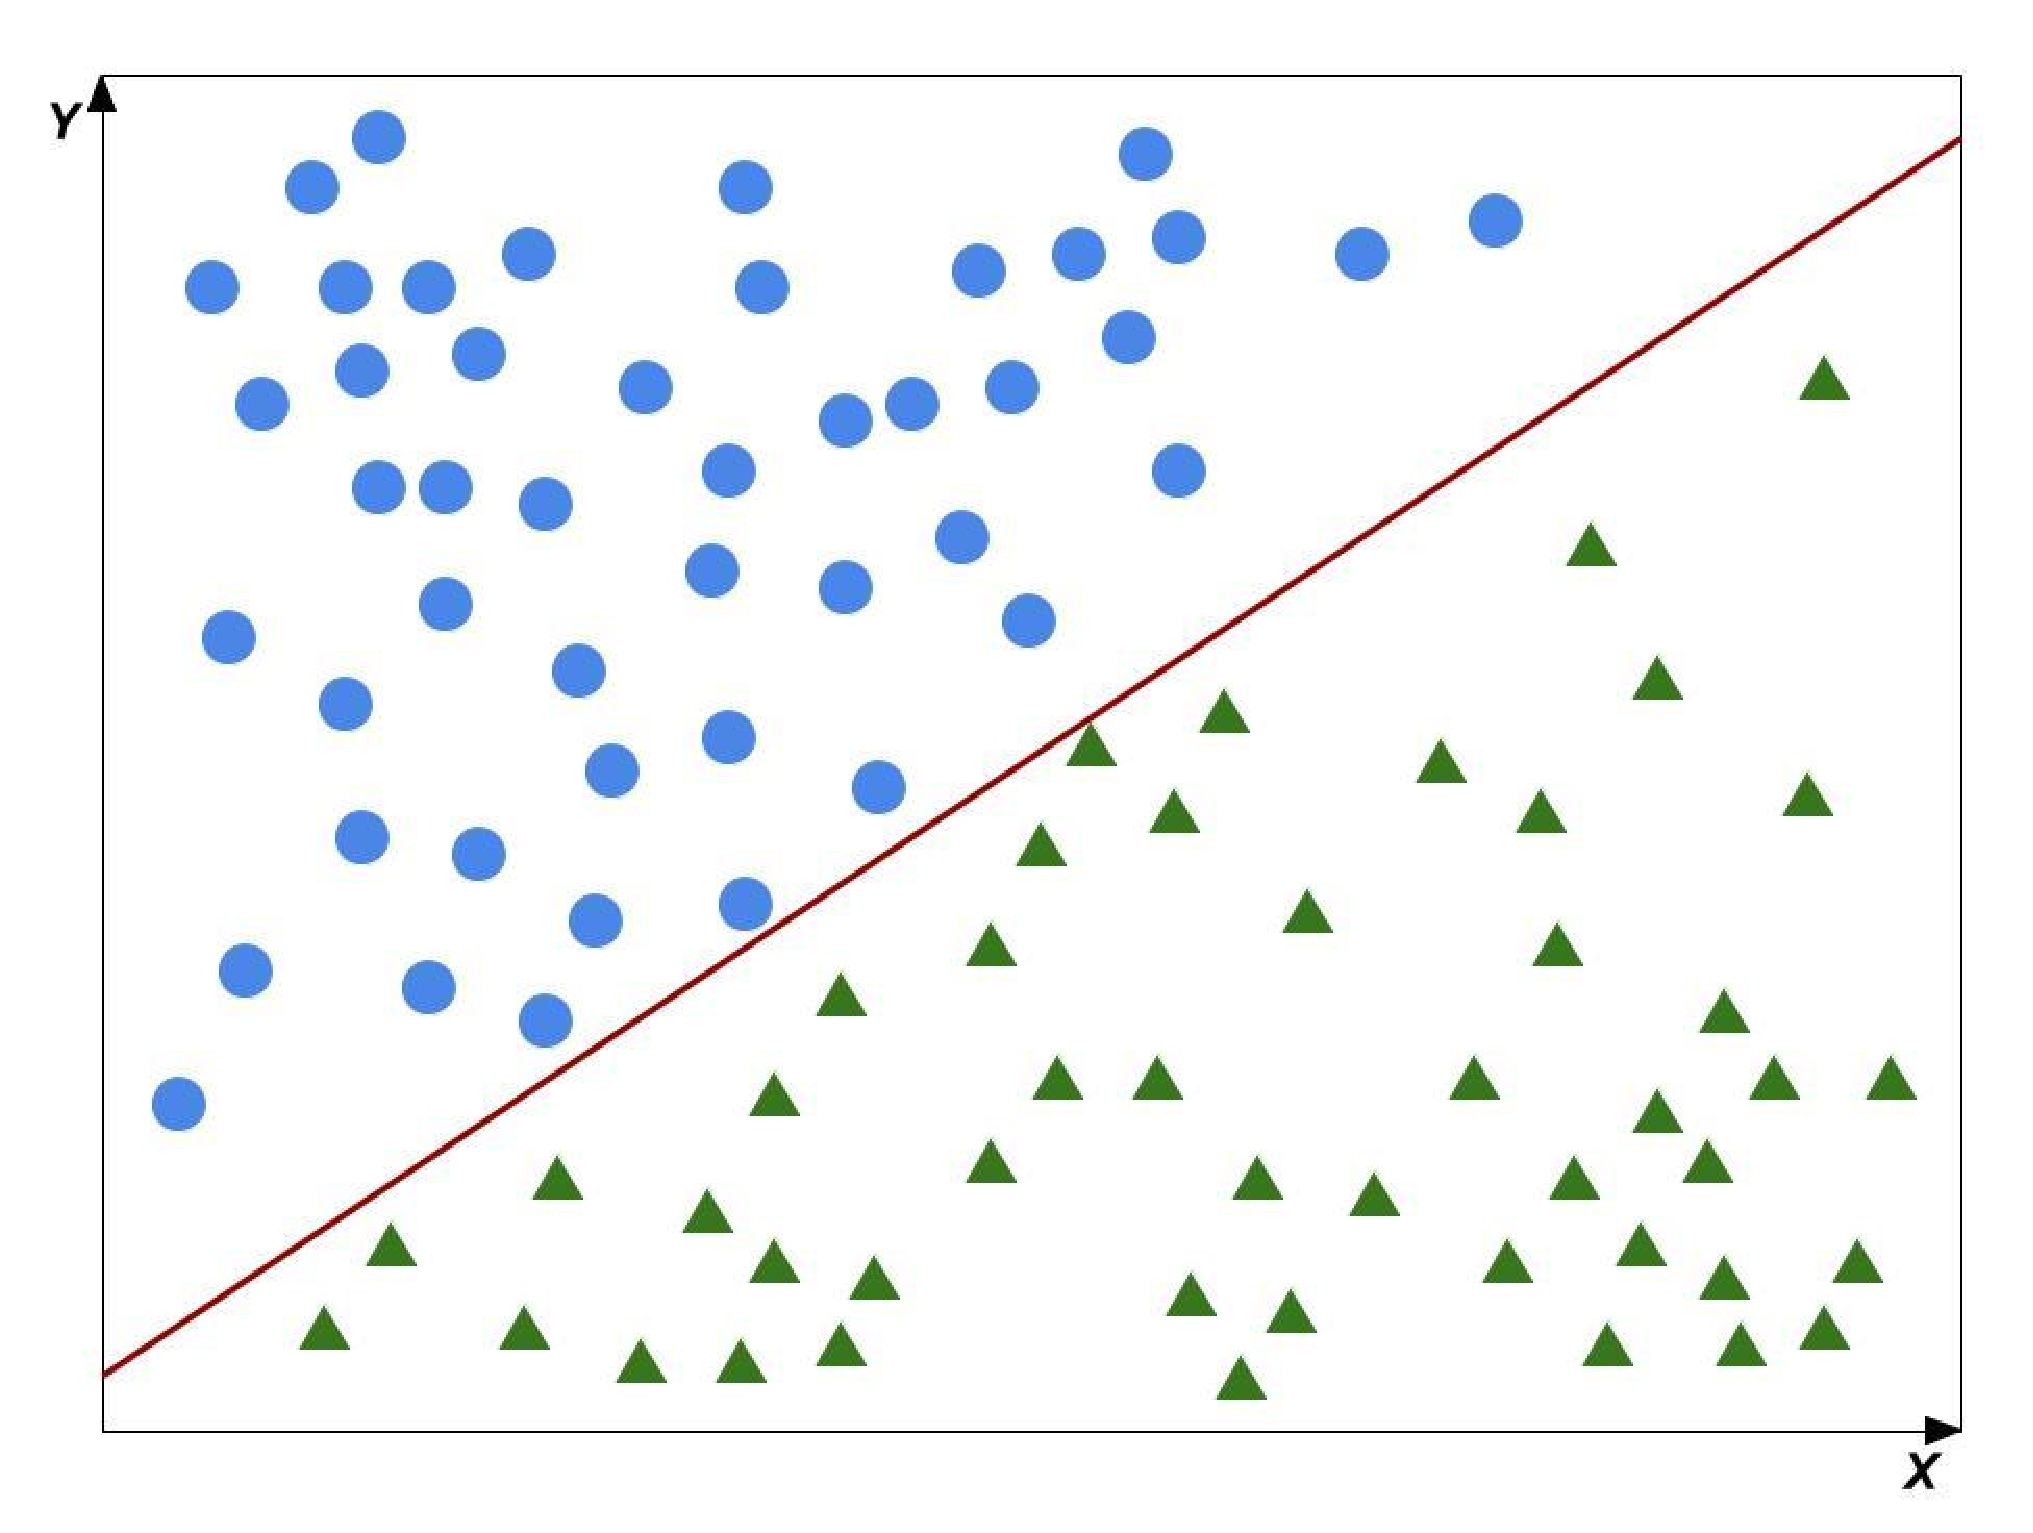
\includegraphics[width=\linewidth]{images/conceitosbasicos02.eps}
  \caption{Exemplo de separador linear}
  \label{fig:conceitosbasicos02}
\end{figure}

Com isso o problema se resume a calcular os valores do vetor de pesos \textit{w}.
Considere que temos disponível os dados dos diversos exemplos de círculos e triângulos vistos na Figura.
Os exemplos envolvidos no processo de aprendizado são denominados \textit{conjunto de dados}.
Cada exemplo contém as coordenadas \textit{(x,y)} mais o valor da classe (circulo ou triângulo).
O algoritmo supervisionado simples proposto a seguir para resolver este problema é baseado no perceptron.
\\

\hline
\begin{center}
\textbf{Algoritmo de aprendizado}
\end{center}
\hline
\hfill \break
Inicializa o vetor \textit{w} com valores aleatórios.
Para cada exemplo do conjunto de dados:
\begin{enumerate}
\item Calcula o valor de saída de \textit{f(x)}
\item Calcula a diferença entre o valor obtido e o real (retirado do exemplo) 
\item Corrige os valores do vetor de pesos \textit{w} por valores proporcionais a esta diferença
\end{enumerate}
\hline
\hfill \break

No exemplo todos os atributos eram números reais.
Porém, com a utilização de outros algoritmos os atributos podem ser de diversos tipos: nominal (uma lista de classes), numérico (um número inteiro ou real), uma data, etc.

As tarefas de aprendizado supervisionado mais clássicas são a classificação, vista no exemplo, e a regressão.
Quando o alvo da tarefa é um atributo nominal dizemos que esta é uma classificação e quando é um número real dizemos que é uma regressão.
Todavia existem outras tarefas nas quais o aprendizado supervisionado pode ser empregado, como é o caso do \textit{ranking}.

Em um problema de \textit{ranking}, queremos que o modelo gere uma lista ordenada de classes como saída.
Para tanto, os exemplos fornecidos ao algoritmo de aprendizado também devem ter uma lista ordenada de classes ao invés de um atributo classe único.
Isto é, em cada exemplo $ (x_i,\; y_i) $ temos que $y_i$ é da forma $ [l_1, l_2, ..., l_k] $ onde \textit{k} representa o número total de classes.

As Tabelas \ref{tab:exdados1} e \ref{tab:exdados2} dão exemplos de dados que podem ser usados para classificação comum e para \textit{ranking} respectivamente.
Os dois exemplos apresentam um certo número de atributos numéricos que podem ser usados pelos algorítimos de aprendizado.
Porém eles diferem no atributo classe, o primeiro tem apenas uma classe enquanto o segundo uma lista.

\begin{table}[h!]
  \begin{center}
    \begin{tabular}{ccccc}
      \textbf{Atributo 1} & \textbf{Atributo 2} & ... & \textbf{Atributo k} & \textbf{Classe} \\
      \hline

      3,14 & 166,55 & ... & -17 & Nodo 10 \\

    \end{tabular}
    \caption{Exemplo de dados para classificação}
    \label{tab:exdados1}
  \end{center}
\end{table}

\begin{table}[h!]
  \begin{center}
    \begin{tabular}{ccccc}
      \textbf{Atributo 1} & \textbf{Atributo 2} & ... & \textbf{Atributo z} & \textbf{Lista de Classes} \\
      \hline

      42 & -33,33 & ... & 0,8 & Nodo 2, Nodo 9, Nodo 5 \\

    \end{tabular}
    \caption{Exemplo de dados para \textit{ranking}}
    \label{tab:exdados2}
  \end{center}
\end{table}

\subsection{Algoritmos de aprendizado}

O perceptron, cujo princípio de funcionamento é o mesmo do algoritmo apresentado anteriormente, é um algoritmo de aprendizado supervisionado clássico encontrado na literatura \cite{Rosenblatt}.
Ele serviu como base para métodos mais complexos como por exemplo o \textit{Support Vector Machine} (SVM) \cite{Chang}.
Entretanto, existem algoritmos baseados em outros princípios.
Quando realizamos os experimentos deste trabalho procuramos comparar classificadores com princípios de funcionamento distintos.
Foram usados os classificadores: SVM, \textit{Naive Bayes} \cite{Murphy}, Arvore de Decisão \cite{Quinlan}, \textit{Random Forest} \cite{Breiman} e \textit{k-nearest neighbors} (KNN) \cite{Duda}.
Descreveremos a seguir de forma breve como esses algoritmos funcionam.

\textbf{Support Vector Machines}.

Como foi dito, o SVM é derivado diretamente do Perceptron.
Ambos são classificadores binários lineares não probabilísticos.
O SVM também pode ser usado para resolver problemas como o da Figura \ref{fig:conceitosbasicos02}.
Este classificador considera cada vetor de atributos de entrada \textit{x} com \textit{d} dimensões.
Ele então calcula um hiperplano, com \textit{d-1} dimensões, para separar os pontos no espaço \textit{d}-dimensional dos exemplos.
No exemplo da Figura temos que \textit{d} é igual a 2 e portanto o hiperplano é uma reta.
Este calculo ocorre iterativamente, a partir do conjunto de treino, de forma análoga ao algorítimo apresentado anteriormente.
Além disso, o SVM procura encontrar o melhor hiperplano de separação para os pontos, i.e. aquele mais afastado de todos. 
Para tanto ele considera a existência uma \texiit{margem} que representa o afastamento do hiperplano para os pontos.
Por fim ele calcula o hiperplano de margem máxima.

\textbf{Naive Bayes}.

\textit{Naive Bayes} são classificadores probabilísticos baseados no teorema de Bayes.
Este algoritmo cria um modelo de probabilidade condicional que recebe como entrada o vetor $ \textit{x} = (x_1, x_2, ... , x_d) $, com \textit{d} atributos.
Ele assume entretanto que estes atributos de entrada são independentes.
Para classificar uma instância o modelo determina a probabilidade de cada classe $C_i$ possível, dada por $p(C_i|x_1, x_2, ... , x_d)$, com a ajuda do teorema de Bayes.
Por fim, o classificador utiliza as probabilidades para decidir qual classe escolher baseado em uma regra preestabelecida, e.g. a classe mais provável.

\textbf{Árvores de Decisão}.

As Árvores de Decisão são modelos de predição que utilizam os atributos de entrada para tomar decisões e desta forma inferir a classe de uma instância.
Sendo assim, as folhas da árvore representam classes enquanto os nodos representam decisões baseadas nos atributos.
De forma geral, para construir um modelo a partir do conjunto de treino, a árvore de decisão escolhe a cada nodo o atributo que melhor divide o conjunto.
Depois que o modelo está pronto, é possível utilizar os atributos de uma nova instância para percorrer a árvore de acordo com as decisões nos nodos.
Com isso chega-se até uma folha que determinará a classe da instância.
Note que tipos distintos de árvore podem utilizar critérios diferentes para a escolha do atributo decisório dos nodos.
O \textit{ Ganho de Informação} por exemplo é empregado nas arvores de decisão do tipo C4.5 (utilizadas nos testes conduzidos neste trabalho).

\textbf{Random Forest}.

O \textit{Random Forest} é um método que utiliza um comitê de árvores de decisão para classificação.
Isto é, durante o treinamento o algoritmo cria diversas árvores de decisão que compõem o modelo.
Cada árvore contribui votando em uma classe e no final a classe mais votada é escolhida.
Esse algoritmo utiliza \textit{Bagging} para criar subconjuntos aleatórios do conjunto de treino.
Cada subconjunto é utilizado para treinar uma das árvores de decisão.
Além disso, o \textit{Random Forest} também emprega o \textit{Feature Bagging}, i.e. cada árvore utiliza somente um subgrupo aleatório dos atributos originais no treinamento.


\textbf{k-Nearest Neighbors}.

O algoritmo \textbf{KNN} apenas recebe os vetores de atributos de entrada do conjunto de treino em um primeiro momento.
Para classificar uma instância ele simplesmente determina qual é a classe mais frequente entre os \textit{k} exemplos mais próximos, onde \textit{k} é definido pelo usuário.
Este método pode utilizar diferentes métricas de proximidade para determinar os vetores próximos, uma das mais utilizadas é a distância euclidiana.

\subsection{Avaliação de Performance}

Para treinar e avaliar a performance de um algoritmo de aprendizado, tipicamente o conjunto de dados é dividido em dois.
O primeiro, \textit{conjunto de treino}, contém os exemplos que efetivamente serão usados para treinar o algoritmo.
O restante, \textit{conjunto de testes}, é usado para fornecer exemplos inéditos ao modelo.
O resultado obtido quando o conjunto de testes é submetido ao modelo é utilizando para calcular as métricas pertinentes.
Essa divisão de dados é feita para garantir que o modelo foi capaz de generalizar e não apenas decorou o conjunto de dados (\textit{overfitting}).
Note que esta técnica de avaliação acaba por não utilizar uma parte dos dados (conjunto de teste) no treinamento.
Isso pode criar dificuldades quando a quantidade de dados disponível for muito limitada.

Outra forma de avaliação importante é chamada \textit{validação cruzada}.
Neste caso o conjunto de dados é dividido em \textit{k} subconjuntos.
Estes podem ou não manter aproximadamente as mesmas proporções de classes do conjunto de dados original, dependendo do que se deseja fazer.
A partir disso o algoritmo de aprendizado é executado \textit{k} vezes, gerando um modelo diferente por vez.
A cada iteração, aquele modelo é treinado com \textit{k-1} subconjuntos como conjunto de treino e o restante (1 subconjunto) como conjunto de testes.
Desta forma, no decorrer das \textit{k} iterações do treinamento, todos os dados são usados.
Por fim, os resultados de todos os modelos são combinados para gerar as estatísticas finais.

\subsection{Métricas de Avaliação}

Para explicar as métricas de avaliação suponha um exemplo onde temos um modelo \textit{M}.
Ele foi treinado para identificar se uma máquina apresenta falha ou não, baseando-se em uma série de medidas recolhidas sobre a mesma (atributos).
Aplicamos então esse modelo à um conjunto de 100 instâncias e obtemos um resultado como o da Tabela \ref{tab:positivosenegativos}.

\begin{table}[h!]
  \begin{center}
    \begin{tabular}{ccc}
      \hline
        & \textbf{Real: com falha} & \textbf{Real: sem falha} \\
      \hline

      \textbf{Previsto: com falha} & 5 (\textit{true positive}) & 5 (\textit{false positive}) \\
      \textbf{Previsto: sem falha} & 10 (\textit{false negative}) & 80 (\textit{true negative} )\\

      \hline
    \end{tabular}
    \caption{Resultados do modelo \textit{M}}
    \label{tab:positivosenegativos}
  \end{center}
\end{table}

Os dados da Tabela \ref{tab:positivosenegativos} estão separados em \textit{true positive} (TP), \textit{true negative} (TN),\textit{false positive} (FP) e \textit{false negative} (FN).
Os dois primeiros indicam o número de instâncias corretamente classificadas e o restante a quantidade classificada incorretamente.
Isto é, \textit{TP} é o número de instâncias que foram classificadas como sendo da classe "com falha" e que realmente pertencem à essa classe.
Já \textit{TN} é o número de instâncias de outras classes, no exemplo temos somente "sem falha", que foram classificados corretamente.
Em contraste, \textit{FP} é a quantidade de instâncias que são da classe "com falha" mas que foram classificadas como sendo de outras classes.
Por fim, \textit{FP} é a quantidade de instâncias da classe "sem falha" que foram erradamente classificadas como sendo "com falha".


A partir desses valores é possível gerar algumas das métricas mais usuais em aprendizado de máquina, as quais apresentaremos nas equações a seguir.

\begin{align*}

\[ \textit{Acurácia} &= \frac{TP+TN}{TP+TN+FP+FN} \] \\
\[ \textit{Precision_i} &= \frac{TP_i}{TP_i+FP_i} \] \\
\[ \textit{Recall_i} &= \frac{TP_i}{TP_i+FN_i} \]
\end{align*}

Conforme as métricas foram apresentadas temos que a \textit{Acurácia} tem um valor único para o modelo.
Contudo o \textit{Precision} e o \textit{Recall} se referem à uma classe por vez.
Note que no exemplo temos duas classes: "com falha" e "sem falha".
Logo, baseando-se nas equações, temos no exemplo da Tabela \ref{tab:positivosenegativos} um valor de \textit{Acurácia} igual a 85\%.
Para classe "com falha" temos o \textit{Precision} igual a 50\% e \textit{Recall} igual a 33,33\%.

Notadamente cada uma dessas métricas é mais apropriada em casos distintos.
A \textit{Acurácia} talvez seja a métrica mais intuitiva e simples, visto que ela representa a proporção de elementos corretamente classificados.
Mas nem sempre é possível avaliar um modelo da melhor maneira com ela.
Considere por exemplo o caso de um modelo \textit{M'} que simplesmente classifica as instâncias como \textit{sem falha}.
Ele atingiria uma \textit{Acurácia} de 85\% mas seria incapaz de identificar máquinas com falha, seu \textit{Recall} para classe "com falha" seria zero.

Generalizações dessas métricas para problemas multiclasse encontradas na literatura são denominadas \textit{Macro Precision} e \textit{Macro Recall}.
Neste caso as métricas são calculadas normalmente para cada classe, mas no final é tirada uma média aritmética.
Apresentamos a seguir as fórmulas dessas outras formas de calcular as métricas.
Nestas fórmulas considere que \textit{k} é o número de classes do conjunto de dados e que $TP_i$, $FP_i$, e $FN_i$ se referem à classe \textit{i}.

\begin{align*}

\[ \textit{Macro Precision} &= \frac{\sum_{i=1}^{k} \frac{TP_i}{TP_i+FP_i}}{k} \] \\
\[ \textit{Macro Recall} &= \frac{\sum_{i=1}^{k} \frac{TP_i}{TP_i+FN_i}}{k} \]

\end{align*}

A Tabela \ref{tab:positivosenegativos2} mostra mais um exemplo, agora com três classes: A, B e C.
Neste exemplo, para calcular o \textit{Precision} para classe A, devemos proceder conforme demonstrado a seguir.

\begin{align*}

\[ \textit{Precision_A} &= \frac{TP_A}{TP_A+FP_A} \] \\
\[ \textit{Precision_A} &= \frac{30}{30+10+5} \] \\

\end{align*}

As demais métricas podem ser calculadas de forma análoga aplicando-se as fórmulas.
Seus valores são apresentados na Tabela \ref{tab:resultados_exemplo2}.

\begin{table}[h!]
  \begin{center}
    \begin{tabular}{cccc}
      \hline
        & \textbf{Real: A} & \textbf{Real: B} & \textbf{Real: C}\\
      \hline

      \textbf{Previsto: A} & 30 & 10 & 5 \\
      \textbf{Previsto: B} & 5 & 25 & 5 \\
      \textbf{Previsto: C} & 5 & 0 & 15 \\

      \hline
    \end{tabular}
    \caption{Exemplo com três classes}
    \label{tab:positivosenegativos2}
  \end{center}
\end{table}

\begin{table}[h!]
  \begin{center}
    \begin{tabular}{ccccc}
      \hline
        & \textbf{Classe A} & \textbf{Classe B} & \textbf{Classe C} & \textbf{Macro}\\
      \hline

\textbf{Precision}	&	66.67	&	71.43	&	75	&	71.03	\\
\textbf{recall}	&	75	&	71.43	&	60	&	68.81	\\

      \hline
    \end{tabular}
    \caption{Exemplo com três classes}
    \label{tab:resultados_exemplo2}
  \end{center}
\end{table}

Para compreender intuitivamente o \textit{Precision} e o \textit{Recall} podemos recorrer à conceitos de \textit{Information Retrieval}.
Neste contexto o \textit{Precision} denota qual proporção dos elementos selecionados pelo modelo realmente são relevantes, no caso do exemplo da Tabela \ref{tab:positivosenegativos} máquinas com falha.
Por outro lado, o \textit{Recall} representa qual proporção dos elementos relevantes presentes nos dados foi selecionada pelo modelo.

Também é importante compreender essas métricas no contexto do problema da rede, onde precisamos enviar equipes para corrigir as falhas.
Podemos entender o $Precision_i$ como o número de vezes que equipes são enviadas ao nodo \textit{i} e ele falhou, dividido pelo número de vezes total que equipes são enviadas à este nodo.
Por outro lado, o $Recall_i$ é o número de vezes que equipes são enviadas ao nodo \textit{i} e ele falhou, dividio pelo número total de vezes que este nodo falhou.
